\section{Introduzione}

L'applicazione \textit{ltspice2circuitikz} permette di convertire un file proveniente dal simulatore \textit{LTSpice} (file .asc) in un documento contente il codice latex che rappresenta il circuito simulato. Inoltre, è in grado di mostrare un file pdf che mostra il circuito corrispondente al codice latex generato e, nel caso di errori di formattazione del file in ingresso, è possibile mostrare un file .asc formattato nel modo corretto. 

\section{Installazione}
L'applicazione è disponibile solo per PC Windows. Per installare l'applicazione è sufficiente decomprimere la cartella compressa \textit{"ltspice2circuitikz app.zip"}. Una volta decompressa, assicurarsi che il contenuto della cartella sia il seguente (figura \ref{fig:contenuto}):

\begin{figure}[h!]
	\centering
	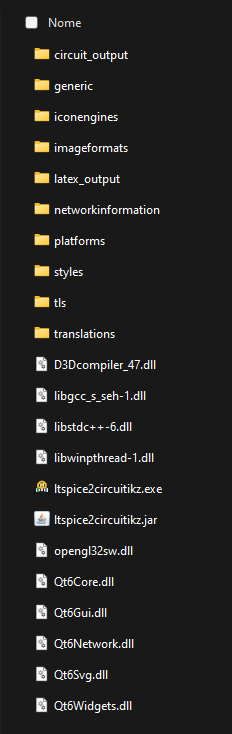
\includegraphics[width=0.25\textwidth]{./ImageFiles/contenuto.png}
	\caption{Contenuto della cartella \textit{"ltspice2circuitikz app.zip"}.}
	\label{fig:contenuto}
\end{figure}

L'applicazione è stata realizzata utilizzando le librerie Qt e l'ambiente di sviluppo Qt IDE. Il componente che si occupa di eseguire la verifica e la traduzione, invece, è stato realizzato in Java. Per il corretto funzionamento dell'applicazione è necessario che sul PC sia installato Java. Per lanciare l'applicazione è sufficiente cliccare due volte sul programma \textit{ltspice2circuitikz.exe}.

\section{Funzionalità}
L'applicazione \textit{ltspice2circuitikz} permette di convertire i circuiti generati con il simulatore LTSpice in documenti latex che utilizzano il package \textit{CircuiTikz} per disegnare il circuito in questione. In figura \ref{fig:schema} sono mostrati i file di input e output dell'applicazione. 
\begin{figure}[h!]
	\centering
	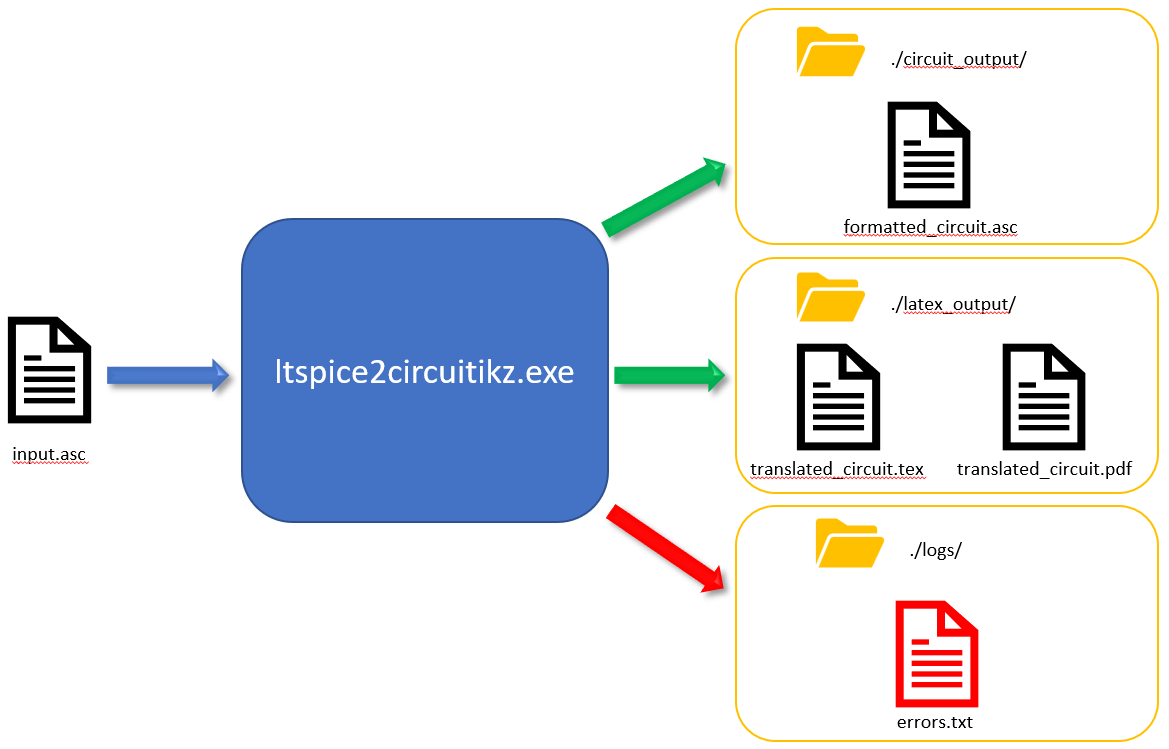
\includegraphics[width=1\textwidth]{./ImageFiles/schema funzionamento.png}
	\caption{File in input e output dall'applicazione.}
	\label{fig:schema}
\end{figure}
Dopo aver generato un file con estensione .asc tramite il simulatore LTSpice, è possibile selezionare tale file per la generazione del circuito in latex. L'applicazione \textit{ltspice2circuitikz} analizza il file in ingresso alla ricerca di errori sintattici e/o semantici. Nel caso in cui non siano presenti errori, viene eseguita la traduzione e vengono generati tre file:
\begin{itemize}
	\item \textit{translated\_circuit.tex}: contiene il testo in latex che utilizza il package \textit{CircuiTikz} per generare il circuito in un documento latex;
\end{itemize}

\todo{continua con la spiegazione dei file che genera. aggiungere anche la funzionalità che gira il circuito se [ più largo che lungo]}


\section{Esempio}





